
\chapter{Framework automatic tuning \label{chap:Framework-parameter-tuning}}

% First paragraph has no indentation.

The assessment of the radio coverage is essential for network planning
and optimization. Consequently, the planning tools used to gather
this information play a key role in the decisions made during the
planning phase of a radio network. But acquiring the necessary information
to support the decision making in this context is a challenging task.
Particularly, planning tools have to be adapted for a specific environment
and technology in order to improve their accuracy. The complexity
of this problem means that radio-coverage prediction is generally
a computationally-intensive and time-consuming task, hence the importance
of fast and accurate prediction tools.

Within this context, we present an open-source simulation framework
for planning and optimization of radio networks. We provide two use
cases for the newly deployed LTE network in Slovenia. The first one
involves the parameter tuning of an empirical radio-propagation model
using a snapshot of field measurements. The other one involves the
optimization of clutter losses over different regions of the country,
therefore adapting the losses due to land usage to the local conditions
of each region.

We report the results of our experimental simulations over three regions
of the real LTE network, deployed by Telekom Slovenije, d.d., thus
showing the suitability of the parallel framework for tackling real-world
planning and optimization problems.


\section{Introduction}

With the advent of long-term evolution (LTE) as the fourth generation
(4G) in cellular technology, mobile operators are facing the challenges
of deploying a new network. LTE follows the well established universal
mobile telecommunication system/high-speed packet access (UMTS/HSPA)
combo, targeting higher peak data rates, higher spectral efficiency
and lower latency \cite{Song_Evolved_cellular_network_planning_and_optimization_for_UMTS_and_LTE:2010}. 

The deployment of a new mobile network is always a challenge for mobile
operators, who constantly struggle to find the optimal investment
in order to provide a competitive network in terms of coverage and
quality of service. Indeed, coverage planning remains a key problem
that all operators have to deal with. It has proven to be a fundamental
issue since the deployment of the first GSM networks, more than 20
year ago.

One of the primary objectives of radio-coverage planning is to efficiently
use the allocated frequency band for a geographic area to be satisfactorily
reached with the radio stations of the network. To this end, radio-coverage
prediction tools are of great importance as they allow network engineers
to test different configurations before physically implementing the
changes. However, to accurately predict the radio coverage of a mobile
network is a very complex task, mainly due to the wide range of various
combinations of hardware and configuration parameters which have to
be analyzed in the context of different environments. The complexity
of the problem means that radio-coverage prediction is generally a
computationally-intensive and time-consuming task, hence the importance
of fast and accurate prediction tools.

Although different mathematical models have been proposed for radio-propagation
modeling, none of them excels in a network-wide scenario \cite{Shabbir_Comparison_of_radio_propagation_models:2011}.
Empirical propagation models usually give good results with a limited
computational effort. However, for improved accuracy, the model parameters
have to be adapted to better fit a specific network or region within
it, mainly because of inaccuracies in input data and environmental
changes in the network region, e.g. foliage of trees or snow. Consequently,
a combination of different parameters is generally needed in order
to reliably calculate radio-propagation predictions for particular
environments. Moreover, since the number of deployed cells (transmitters)
keeps growing with the adoption of modern standards \cite{Saleh_On_the_coveraga_extension_in_LTE_networks:2010},
there is a clear need for a radio propagation tool that is able to
cope with larger work loads in a feasible amount of time.

To address the afore-mentioned issues, we adapt the parameters of
an empirical propagation model to a set of field measurements. The
parameter tuning is analytically calculated per cell, in order to
increase the accuracy of the calculated predictions. Moreover, we
fine tune the signal losses due to land usage (clutter) in a regional
basis, using an optimization approach. As a working framework to tackle
the presented problems, we use a parallel radio-prediction tool \cite{Benedicic-A_GRASS_GIS_parallel_module_for_radio-propagation_predictions:2013},
thus showing the suitability of the presented framework for real-world
planning and optimization of LTE radio networks. Particularly, we
show the tool capabilities to handle several parallel radio-prediction
runs using a metaheuristic algorithm and distributed objective-function
evaluation, while resolving the clutter optimization problem.

This paper is organized as follows. Section \ref{sec:Simulation-framework}
gives a description of the parallel simulation framework, including
some implementation details and performance figures. Section \ref{sec:Radio-propagation-prediction}
introduces principles of radio-propagation prediction, and the mathematical
model used. The parameter-tuning problem and the analytical approach
for tackling it are presented in Section \ref{sec:Parameter-tuning},
including the simulations performed on the framework and their results.
Section \ref{sec:Clutter-optimization} concentrates on describing
the optimization problem involving the regional adaptation of signal
losses due to clutter, including the performed simulations the achieved
results. Finally, Section \ref{sec:Related-work} gives an overview
of relevant publications, describing how they relate to our work,
before drawing some conclusions.


\section{Simulation framework}\label{sec:Simulation-framework}

As if was mentioned before, we use the parallel radio-prediction tool
PRATO \cite{Benedicic-A_GRASS_GIS_parallel_module_for_radio-propagation_predictions:2013}
as our simulation and optimization framework. PRATO deals with complex
calculations over large data sets by applying a work-pool parallel
paradigm over a message-passing communication model. As such, PRATO
is ready to be deployed over small groups of networked computers as
well as over a computer cluster with hundreds of nodes. Since the
prediction calculation employs digital elevation models and land-usage
data in order to analyze the radio coverage of a geographic area,
the framework is implemented as a module of the open source Geographic
Resources Analysis Support System (GRASS) \cite{Neteler_Open_source_GIS_a_GRASS_GIS_approach}.


\subsection{Parallel computation on computer clusters}

Considering the high computational power needed for evaluating the
radio coverage of real mobile networks during optimization, the use
of a computer cluster is preferred. A computer cluster is a group
of interconnected computers that work together as a single system.
To reach high levels of parallel performance and scalability, PRATO
performs the parallel decomposition big data sets, distributing the
computational load among the computing nodes that belong to the cluster.

Computer clusters typically consist of several commodity PCs connected
through a high-speed local network with a distributed file system,
like NFS \cite{Shepler_Network_file_system:2003}. One such system
is the DEGIMA cluster \cite{Hamada_Cluster_of_GPUs:2010} at the Nagasaki
Advanced Computing Center (NACC) of the Nagasaki University in Japan.
This system ranked in the TOP 500 list of supercomputers until June
2012%
\footnote{http://www.top500.org%
}, and in June 2011 held the third place of the Green 500 list%
\footnote{http://www.green500.org%
} as one of the most energy-efficient supercomputers in the world.


\subsection{Multi-paradigm parallel programming}

The implementation methodology adopted for PRATO follows a multi-paradigm
parallel programming approach in order to fully exploit the resources
of each of the nodes in a computing cluster. To effectively use a
shared memory multi-processor, PRATO uses POSIX threads to implement
parallelism \cite{Butenhof_Programming.with.POSIX.threads:1997}.
By using POSIX threads, multiple threads can exist within the same
process while sharing its resources. For instance, an application
using POSIX threads can execute multiple threads in parallel by using
the cores of a multi-core processor, or use the system resources more
effectively, thus avoiding process execution-halt due to I/O latency
by using one thread for computing, while a second thread waits for
an I/O operation to complete. 

To use the computing resources of a distributed memory system, such
as a cluster of processors, PRATO uses the Message Passing Interface
(MPI) \cite{Gropp_Using_MPI:1999}. MPI is a message-passing standard,
which defines syntax and semantics designed to function on a wide
variety of parallel computers. MPI enables multiple processes running
on different processors of a computer cluster to communicate with
each other. It was designed for high performance on both massively
parallel machines and on workstation clusters. Its development is
supported by a broadly-based committee of vendors, developers, and
users.


\subsection{Master-worker model}

PRATO follows a master-worker paradigm \cite{Mattson_Patterns_for_parallel_programming:2004},
where the main process, i.e. the master, produces many sub-problems,
which are delivered to be executed by the worker processes. These
sub problems are, in this case, the radio-coverage prediction for
individual cells of the radio network under optimization.

The master process is the only component that should be run from within
the GRASS environment. It is responsible for dynamically starting
the worker processes using the available computing nodes, based on
the amount of network cells for which the coverage prediction should
be calculated. For distributing the work among the worker processes,
the master process dispatches the loaded geographic data, before dispatching
them to the multiple worker processes. In this case, the decomposition
of the data applies to the digital-elevation and the clutter data
only, but it could be applied to any point-based data set, vector
or raster. In the next step, the master process starts a message-driven
processing loop, which main task is to evaluate the radio-coverage
prediction of different transmitters among idle worker processes.

The worker processes, on the other hand, are completely independent
from GRASS, i.e. they do not have to run within the GRASS environment
nor use any of the GRASS libraries to work. This aspect significantly
simplifies the deployment phase to run PRATO on a computer cluster,
since no GRASS installation is needed on the computing nodes hosting
the worker processes. During the result-saving phase, each of the
worker processes sends its results independently from each other,
following an asynchronous and decoupled design. Moreover, worker processes
do this from an independent thread, which runs concurrently with the
radio-prediction evaluation of the next transmitter received from
the master process. The overlap between calculation and communication
achieved by the use of an auxiliary thread completely hides the latency
created by the result-dumping task, and makes better use of the system
resources.


\subsection{Performance}

From the performance point of view, PRATO is capable of reaching levels
of high efficiency, as the following measurements show. 

Figure \ref{fig:weak_scalability_time-1} shows the time measurements
of a weak-scalability experiment. To measure the weak-scalability
properties of PRATO means analyzing the scalability of the parallel
implementation in cases where the workload assigned to each MPI process
(one process per processor core) remains constant as the number of
processor cores, and thus the total size of the problem, is increased.

\begin{figure}
\centering

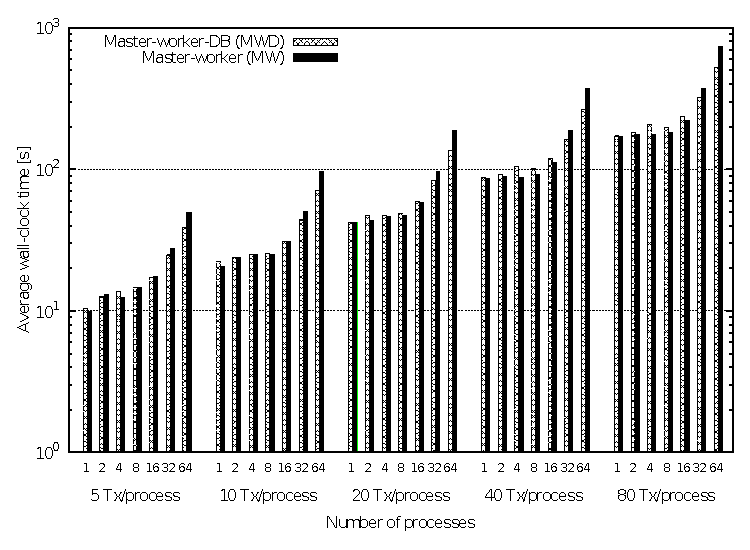
\includegraphics[width=1\columnwidth]{\lyxdot \lyxdot /tun_par/doc/img/weak_scaling-time_plot}

\caption{\textit{\emph{Measured wall-clock time for weak-scalability experiments.}}\textit{
}\textit{\emph{Experiments performed assigned one MPI worker process
per available core. The wall-clock time axis is expressed in base-10
logarithmic scale, whereas the axis representing the number of cores
is expressed in base-2 logarithmic scale.\label{fig:weak_scalability_time-1}}}}
\end{figure}


The time measurements observed from the weak-scalability results show
that the wall-clock times are almost constant for bigger problem instances,
revealing that the achieved level of scalability gets close-to-linear
as the amount of transmitters-per-core increases. Specifically, PRATO
scales especially well when challenged with a big number of cells
or transmitters (10,240 for the biggest instance) over 128 cores.

Another aspect is the strong-scalability capabilities of PRATO, which
represents the performance when increasing the number of computing
cores for a given problem size, i.e. the number of cells deployed
over the target area does not change, while only the number of cores
used is increased. Figure \ref{fig:strong_scalability_speedup-1}
shows the speedup factors achieved for a set of strong-scaling experiments.
We may see that a close-to-linear scaling is achieved, especially
for the biggest problem sizes. Linear scaling occurs when the obtained
speedup is equal to the total number of processors used. However,
it should be noted that perfect speedup is almost never achieved,
due to the existence of serial stages within an algorithm and communication
overheads of the parallel implementation. 

\begin{figure}
\centering

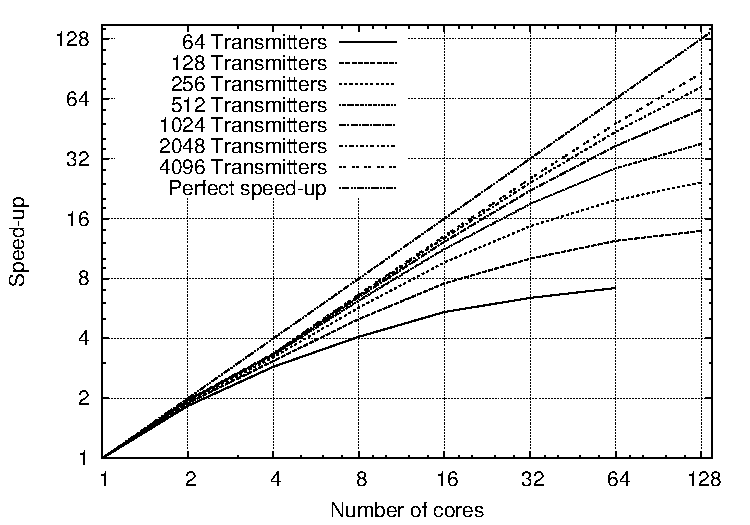
\includegraphics[width=1\columnwidth]{\lyxdot \lyxdot /tun_par/doc/img/strong_scaling-speedup_plot}

\caption{\textit{\emph{Measured speedup for strong-scalability experiments.}}\textit{
}\textit{\emph{The speedup axis is expressed in base-2 logarithmic
scale, whereas the axis representing the number of cores is expressed
in base-2 logarithmic scale.\label{fig:strong_scalability_speedup-1}}}}
\end{figure}


For more detailed information about PRATO, its design and capabilities,
we refer the reader to \cite{Benedicic-A_GRASS_GIS_parallel_module_for_radio-propagation_predictions:2013}.


\section{Radio-propagation prediction}\label{sec:Radio-propagation-prediction}

The objective here is to improve the quality performance of a given
mathematical model, used for radio-propagation calculations, by fine-tuning
its configurable parameters as per-cell basis. In order to do this,
we apply a state-of-the-art analytical approach, based on least squares
method \cite{Yang_A_linear_least_square_method_of_propagation_model_tuning_for_3G_radion_network_planning:2008},
thus combining field measurements to fit the parameters of the mathematical
model.

The idea is to automatically adapt the parameters of the mathematical
model for each of the cells targeted by the optimization. That is,
starting from an a-priori best-known set of parameters, empirically
calculated by the radio engineers at Telekom Slovenije, d.d., this
approach adapts the model parameters so that the deviation of the
radio-propagation prediction to a given set of field measurements
is minimized.

To calculate the radio-coverage predictions we use a mathematical
model based on the well-known empirical Okumura-Hata formula \cite{Hata-Empirical_formula_for_propagation_loss_in_land_mobile_radio_services:1980}.
Other more accurate methods exist, like the ones based on ray tracing
\cite{Corre_Three_dimensional_urban_EM_wave_propagation_model_for_radio_network_planning_and_optimization_over_large_areas:2009,Vilhar-Efficient_open_source_ray_tracing_methods_for_rural_environment:efficient}.
However, these methods are more sensible to deviations in input data,
like digital elevation models and buildings, and are still inefficient
in terms of the computational effort required to achieve satisfying
results.

Empirical methods for radio-propagation predictions, on the other
hand, give acceptable results within a feasible amount of time. For
this reason, they have become the industry standard for non-deterministic
propagation-loss calculations \cite{Aarnaes-Tuning_of_empirical_radio_propagation_models_effect_of_location_accuracy:2004,Begovic_Applicability_evaluation_of_Okumura_Ericsson_and_Winner_propagation_models_for_coverage_planning:2012,Cichon_Propagation.prediction.models:1995,Filiposka_Terrain_aware_three_dimensional_radio_propagation_model_extension_for_NS2:2011,Hata-Empirical_formula_for_propagation_loss_in_land_mobile_radio_services:1980,Ozimek_Open.source.radio.coverage.prediction:2010}.


\subsection{Radio-prediction model\label{sub:Radio-prediction-model}}

The Okumura-Hata model has been largely studied and shown to be suitable
for predicting radio propagation of LTE networks \cite{Ahmad:Studying_different_propagation_models_for_LTE_system:2012}.
Moreover, this mathematical model is especially appropriate for tuning,
as it contains a number of adjustable parameters, which adapt the
model according to a given scenario and its local conditions. In its
primary form, the model distinguishes the distance of receiver from
the transmitter, the frequency used and the effective antenna height,
i.e. the antenna height above the receiver's level, in order to calculate
the path loss in line-of-sight (LOS) conditions. However, the for
distinguishing non-line-of-sight (NLOS) conditions, the terrain profile
and Earth shape are added to the original formula. Moreover, empirical
corrections due to different land usage are also included to improve
the quality of the calculated predictions. Equation (\ref{eq:eric_los})
describes the path loss when there is LOS between the transmitter
and the receiver. 

\begin{multline}
pl_{\mathrm{LOS}}(d_{(x,y)},\beta)=a_{0}+a_{1}\log(d_{(x,y)})+a_{2}\log(H_{A})+\\
a_{3}\log(d_{(x,y)})\log(H_{A})-3.2\left[\log(11.75\cdot H_{R})\right]^{2}+\\
44.49\log(F)-4.78\left[\log(F)\right]^{2},\label{eq:eric_los}
\end{multline}


\noindent where $\beta=(a_{0},a_{1},a_{2},a_{3})$ is the vector containing
the tuning parameters of the model, $d_{(x,y)}$ is the distance (in
kilometers) from the transmitter to the topography point with coordinates
$(x,y)$, $H_{A}$ is the effective antenna height (in meters) of
the transmitter, $H_{R}$ is the antenna height (in meters) of the
receiver, and $F$ is the frequency, expressed in MHz. On the other
hand, in NLOS conditions, the path loss is calculated as in Equation
(\ref{eq:eric_nlos}).

\begin{multline}
pl_{\mathrm{NLOS}}(d_{(x,y)})=\sqrt{\left[\alpha K(d_{(x,y)})\right]^{2}+E(d_{(x,y)})^{2}},\label{eq:eric_nlos}
\end{multline}


\noindent where $\alpha$ is the knife-edge diffraction control parameter,
$K(d_{(x,y)})$ is the knife-edge diffraction loss (in dB) and $E(d_{(x,y)})$
is the correction due to the Earth sphere (in dB). The latter two
values are calculated on the topography point with coordinates $(x,y)$.

In this work, the terrain profile is used for LOS determination. In
order to adequately predict propagation effects due to foliage, buildings
and other fabricated structures, additional loss factors based on
the land usage (clutter data), are included. This technique is adopted
by several propagation models for radio networks \cite{Aarnaes-Tuning_of_empirical_radio_propagation_models_effect_of_location_accuracy:2004,Begovic_Applicability_evaluation_of_Okumura_Ericsson_and_Winner_propagation_models_for_coverage_planning:2012,Neskovic_Microcell_electric_field_strength_prediction_model:2010}.
Consequently, we introduce an extra term for signal loss due to clutter,
thus defining the model-predicted path loss as

\begin{multline}
pl(d_{(x,y)},\beta)=pl_{\mathrm{LOS}}(d_{(x,y)},\beta)+\\
pl_{\mathrm{NLOS}}(d_{(x,y)})+pl_{\mathrm{CLUT}}(d_{(x,y)}),\label{eq:eric_pathloss}
\end{multline}


\noindent where $pl_{\mathrm{CLUT}}(d_{(x,y)})$ is clutter loss at
the topography point with coordinates $(x,y)$, expressed in dB.

In our case, we recognize twelve different clutter categories representing
loss values due to different land usage. These categories, including
their label numbers and descriptions, are depicted in Table \ref{tab:Clutter-categories}.

\begin{table}
\caption{Clutter-category label numbers and their land-usage meanings for the
radio-prediction model. \label{tab:Clutter-categories}}


{\footnotesize \centering}{\footnotesize \par}

{\footnotesize }%
\begin{tabular}{cl}
\hline 
{\footnotesize Clutter category} & {\footnotesize Description}\tabularnewline
\hline 
{\footnotesize 0} & {\footnotesize Urban area without buildings, mostly roads}\tabularnewline
{\footnotesize 1} & {\footnotesize Suburban area }\tabularnewline
{\footnotesize 2} & {\footnotesize Urban area}\tabularnewline
{\footnotesize 3} & {\footnotesize Dense urban area}\tabularnewline
{\footnotesize 4} & {\footnotesize Agricultural area}\tabularnewline
{\footnotesize 5} & {\footnotesize Forestall area}\tabularnewline
{\footnotesize 6} & {\footnotesize Swamp area}\tabularnewline
{\footnotesize 7} & {\footnotesize Dry open land area with special vegetation}\tabularnewline
{\footnotesize 8} & {\footnotesize Dry open land area without special vegetation}\tabularnewline
{\footnotesize 9} & {\footnotesize Water area}\tabularnewline
{\footnotesize 10} & {\footnotesize Industrial area}\tabularnewline
{\footnotesize 11 } & {\footnotesize Park area}\tabularnewline
\hline 
\end{tabular}
\end{table}


In any case, the effectiveness of decision-making during radio-network
planning is tightly coupled with the precision achieved by the propagation
model used. In order to obtain a radio-propagation model that most
accurately reflects the propagation characteristics of the area covered
by each radio cell in the network, the parameters of the mathematical
model are tuned using field-measurement campaigns. Parameter tuning
using this method depends on existing field-measurement data, which
are taken before hand over the area covered by the target network
cells.


\section{Parameter tuning of the radio-prediction model}\label{sec:Parameter-tuning}

The objective here is thus improve the quality performance of a given
mathematical model, used for radio-propagation calculations, by fine-tuning
its configurable parameters as per-cell basis. In order to do this,
we apply a state-of-the-art analytical approach, based on least squares
method \cite{Yang_A_linear_least_square_method_of_propagation_model_tuning_for_3G_radion_network_planning:2008},
thus combining field measurements to fit the parameters of the mathematical
model.

The idea is to automatically adapt the parameters of the mathematical
model for each of the cells targeted by the optimization. That is,
starting from an a-priori best-known set of parameters, empirically
calculated by the radio engineers at Telekom Slovenije, d.d., this
approach adapts the model parameters so that the deviation of the
radio-propagation prediction to a given set of field measurements
is minimized.

In the context of our work, this translates to fine tuning the parameters
of the LOS part of the path-loss prediction model, i.e. $pl_{\mathrm{LOS}}(d_{(x,y)},\beta)$.
The adjustable parameters are the elements of vector $\beta=(a_{0},a_{1},a_{2},a_{3})$,
namely
\begin{description}
\item [{$a_{0}$}] the reference loss or offset;
\item [{$a_{1}$}] the loss slope due to distance of the receiver from
the transmitter;
\item [{$a_{2}$}] the loss slope due to height of the transmitter antenna;
\item [{$a_{3}$}] the loss slope due to the combined effect of the distance
and height of the antenna.
\end{description}
The parameter tuning is performed per cell to improve local fitting
of the radio predictions. The steps to be completed are: collect and
process field-measurement data, and solve the particular system of
linear equations. The resulting solution is the vector $\beta$ of
the target cell, with its values locally adapted.

In the following, we denote the default parameters of the radio-propagation
model with these values
\begin{description}
\item [{$a_{0}$}] 38.0,
\item [{$a_{1}$}] 32.0,
\item [{$a_{2}$}] -12.0, and
\item [{$a_{3}$}] 0.1.
\end{description}

\subsection{Field measurements}

In mobile networks, a moving mobile constantly performs cell selection/reselection
and handover in order to keep the best possible connection to the
network. Within this context, the best connection is selected by measuring
the signal strength or quality of the neighboring cells. In LTE networks,
a mobile measures two parameters on reference signal, namely the Reference
Signal Received Power (RSRP) and the Reference Signal Received Quality
(RSRQ).

For a certain frequency bandwidth, RSRP measures the average received
power over the resource elements that carry cell-specific reference
signals. RSRP is applicable in idle (e.g. waiting for a call) and
connected (e.g. during a call) modes. During the procedure of cell
selection/reselection in idle mode, RSRP is used. On the other hand,
RSRQ is only applicable when the mobile is in connected mode. 

The radio-coverage calculation involves predicting the network coverage
over a certain region, and thus to the users' mobiles within it. Hence,
in the first place, we are interested on accurately predicting the
best connection the mobile would select in idle mode and the RSRP
field measurements it uses.

In our case, the field measurements, representing the RSRP at a given
location, are collected using a small truck equipped with the spectrum
analyzer Rohde \& Schwarz. The spectrum analyzer is connected to an
external omni antenna mounted on the roof of the truck, at roughly
2~meters above the ground, taking measurements at a rate of 50~Hz???,
with the symbol rate set to ???~Mhz. To accurately establish the
measurement location points, a GPS unit was used. The measurement
locations covered most of the streets within the target area, with
over 300,000 individual field-measurement points taken at more of
more than 150 network cells.

To minimize the error impact in measured RSRP and estimated location,
all field measurements are processed so that a single value, the median%
\footnote{The median is the numerical value separating the higher half of a
sample set from the lower half.%
}, is calculated for each of the measured locations. The resulting
RSRP is then used to estimate the path-loss prediction at the location
corresponding to each of the measurements, which resolution matches
those of the digital elevation model and clutter data.


\subsection{Linear least squares}

It is important to note the linear relationship between the predicted
loss $pl(d_{(x,y)},\beta)$ and the components of vector $\beta$,
for this is a necessary condition for the least-squares method to
find a solution. Following this method, the parameter fitting of the
propagation model is based on the minimization of an observed error,
i.e. the sum of the squared difference between the predicted and measured
RSRP,

\begin{multline}
E(c)=\sum_{i=1}^{m_{c}}(p_{c}-pl_{c}(d_{(x,y)},\beta_{c})-fm_{i})^{2},\label{eq:least_squares_error}
\end{multline}


\noindent where $E(c)$ is the observed error for cell $c$, $p_{c}$
is the transmit power of cell $c$, and $fm_{i}$ is the $i$-th field
measurement out of a set of measurements of cell $c$ with cardinality
$m_{c}$.


\subsection{Simulations \label{sub:Simulations}}

The simulations carried out for this part of our work comprise building
the matrices of observed-error values, $E(c)$, for each cell $c$
in the target network. The linear systems of equations are then individually
solved by applying the linear least squares method \cite{Yang_A_linear_least_square_method_of_propagation_model_tuning_for_3G_radion_network_planning:2008},
which involves the evaluation of one radio-coverage prediction per
cell. Each system holds a unique solution for each cell $c$, denoted
by the vector $\beta_{c}$.

\begin{table*}
\caption{Percentage of clutter-category proportions for each of the test networks
used. The category legend is given in Table \ref{tab:Clutter-categories}.
\label{tab:Proportion_of_clutter_for_test_networks}}


{\footnotesize \centering}{\footnotesize \par}

{\footnotesize }%
\begin{tabular}{ccccccccccccc}
\hline 
 & {\footnotesize Cat. 0} & {\footnotesize Cat. 1} & {\footnotesize Cat. 2} & {\footnotesize Cat. 3} & {\footnotesize Cat. 4} & {\footnotesize Cat. 5} & {\footnotesize Cat. 6} & {\footnotesize Cat. 7} & {\footnotesize Cat. 8} & {\footnotesize Cat. 9} & {\footnotesize Cat. 10} & {\footnotesize Cat. 11}\tabularnewline
\hline 
{\footnotesize Net$_{1}$ } & {\footnotesize 0.53} & {\footnotesize 4.53} & {\footnotesize 1.68} & {\footnotesize 0.45} & {\footnotesize 71.89} & {\footnotesize 17.94} & {\footnotesize 0.07} & {\footnotesize 0.00} & {\footnotesize 0.03} & {\footnotesize 2.21} & {\footnotesize 0.67} & {\footnotesize 0.00}\tabularnewline
{\footnotesize Net$_{2}$ } & {\footnotesize 0.91} & {\footnotesize 5.53} & {\footnotesize 9.48} & {\footnotesize 3.84} & {\footnotesize 29.73} & {\footnotesize 48.57} & {\footnotesize 0.14} & {\footnotesize 0.03} & {\footnotesize 0.03} & {\footnotesize 0.76} & {\footnotesize 0.86} & {\footnotesize 0.12}\tabularnewline
{\footnotesize Net$_{3}$ } & {\footnotesize 0.15} & {\footnotesize 3.99} & {\footnotesize 1.14} & {\footnotesize 0.11} & {\footnotesize 26.50} & {\footnotesize 67.13} & {\footnotesize 0.26} & {\footnotesize 0.00} & {\footnotesize 0.00} & {\footnotesize 0.36} & {\footnotesize 0.36} & {\footnotesize 0.00}\tabularnewline
\hline 
\end{tabular}
\end{table*}


\begin{figure*}
\begin{minipage}[t]{0.49\textwidth}%
\centering

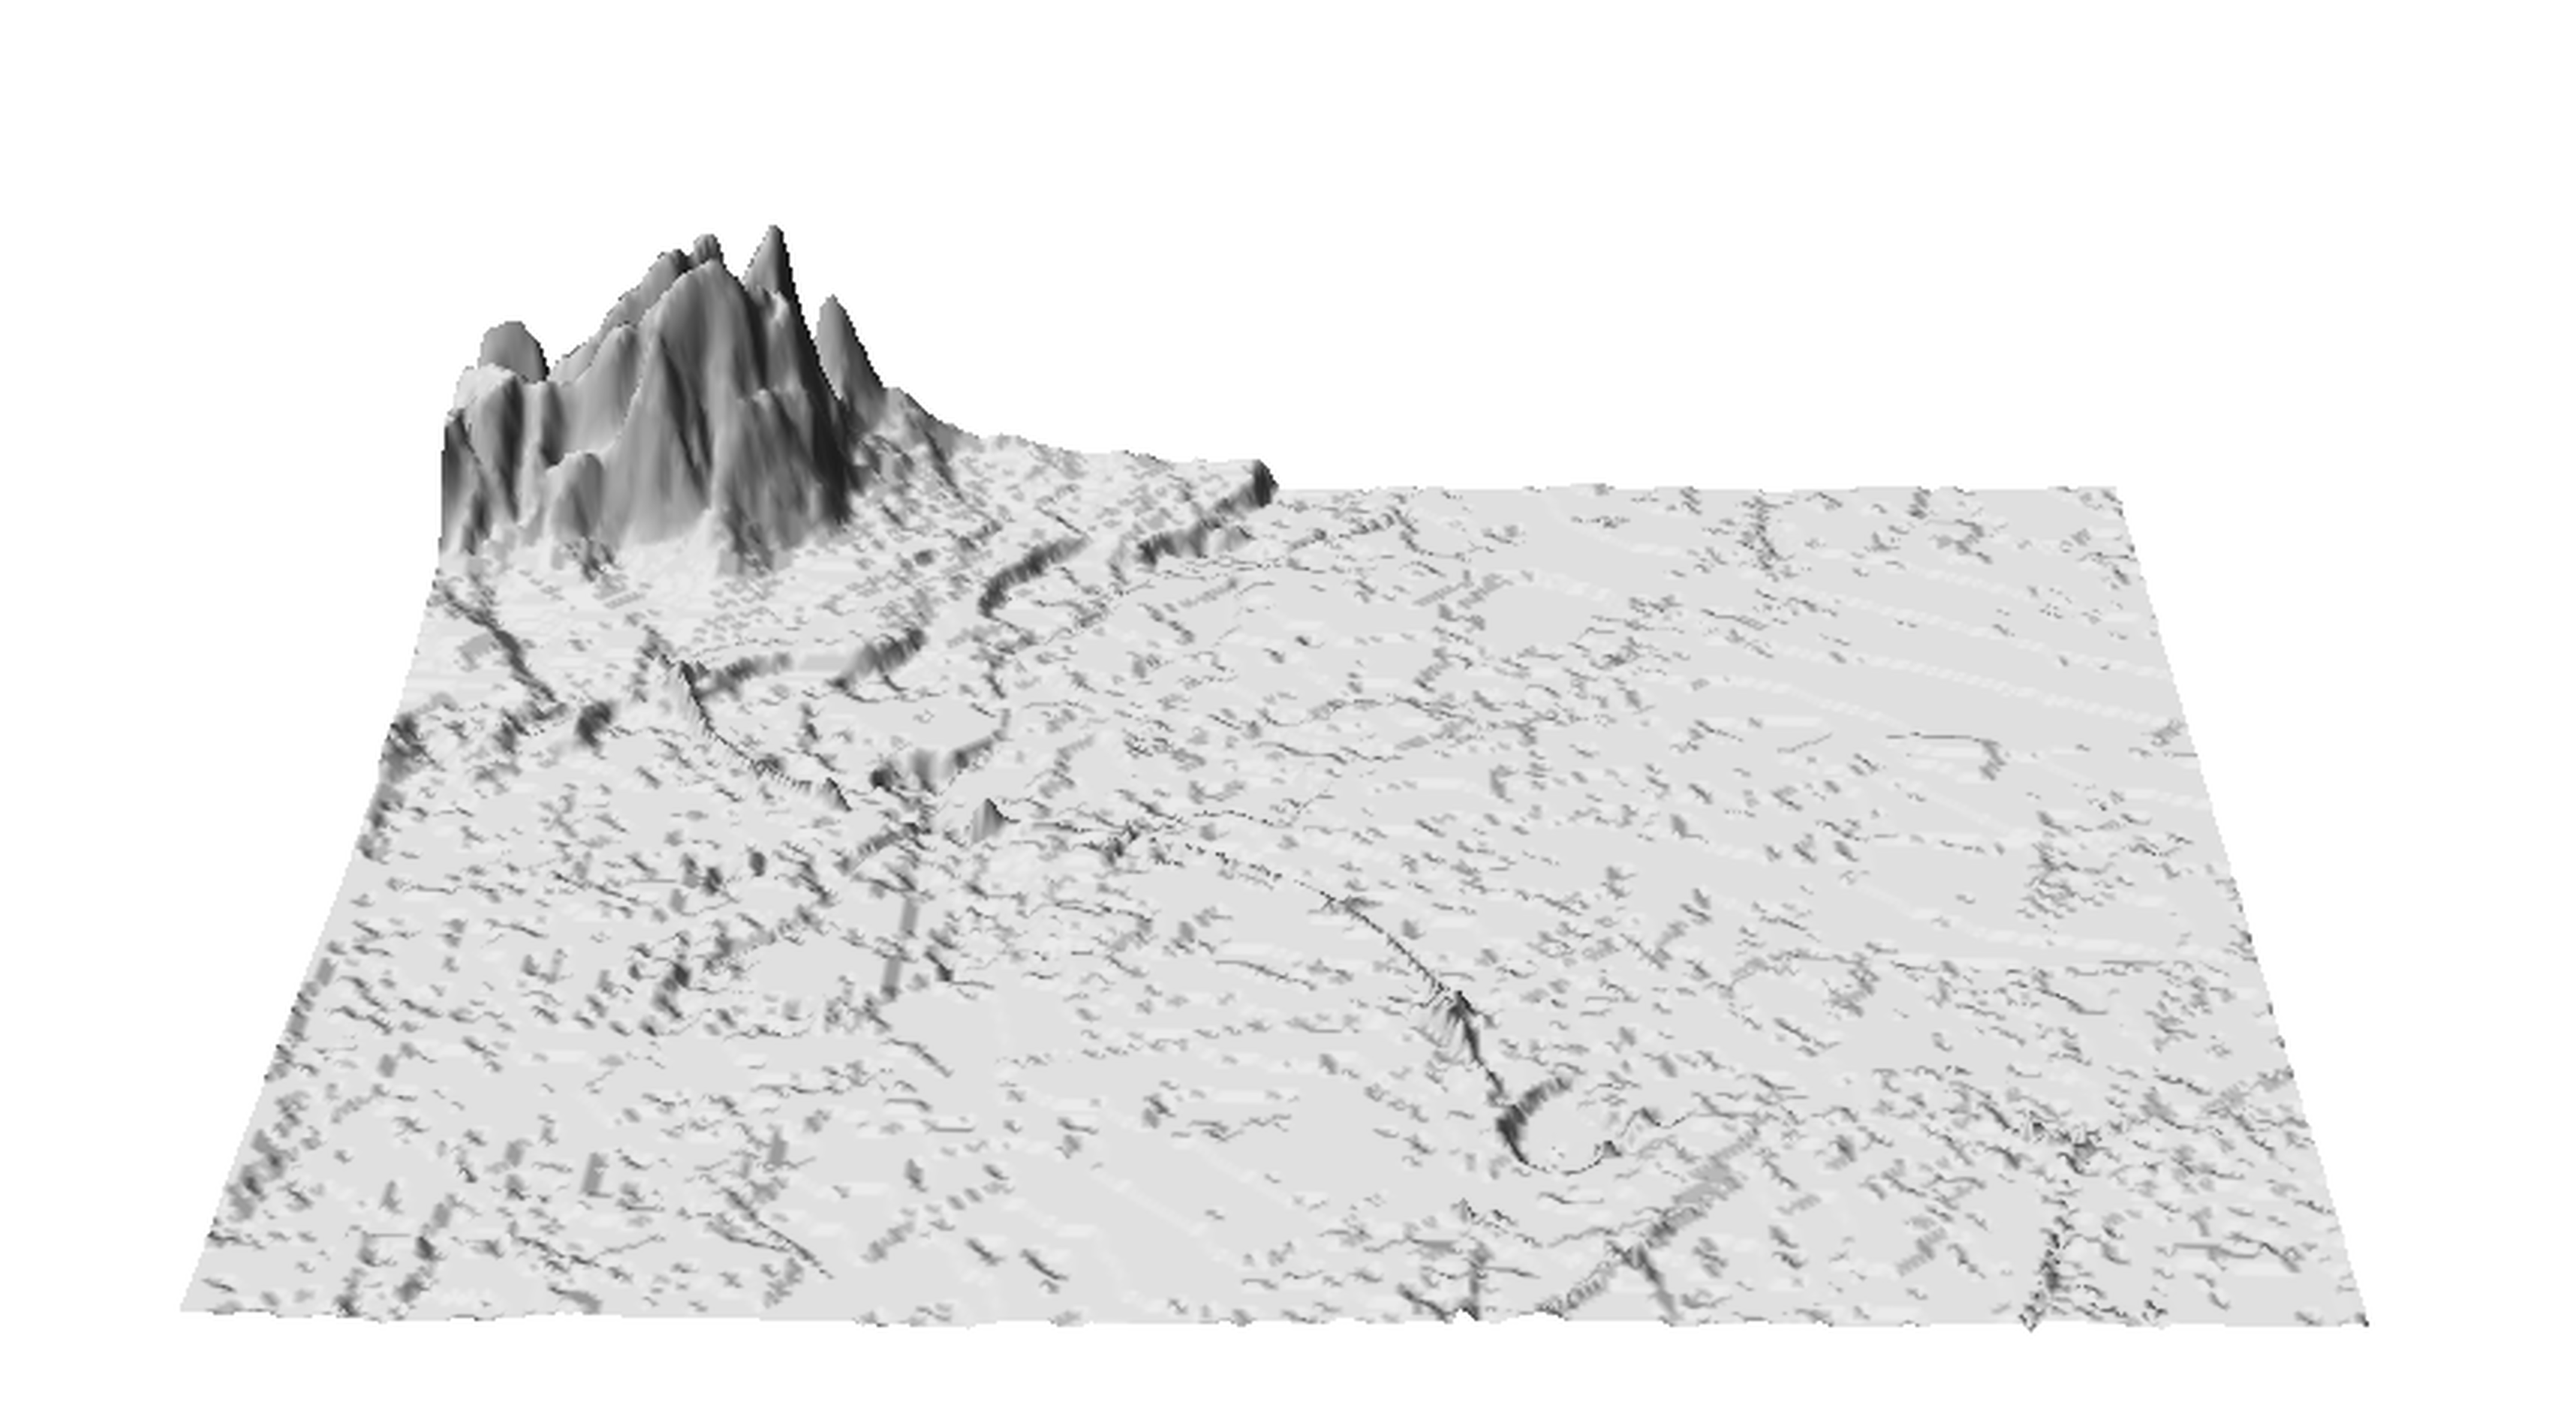
\includegraphics[width=1\columnwidth]{\lyxdot \lyxdot /tun_par/doc/img/terrain_MS}

\caption{Terrain profile for network Net$_{1}$, dominated by an agricultural
area.\label{fig:terrain_profile-Net1}}
%
\end{minipage}\hfill{}%
\begin{minipage}[t]{0.49\textwidth}%
\centering

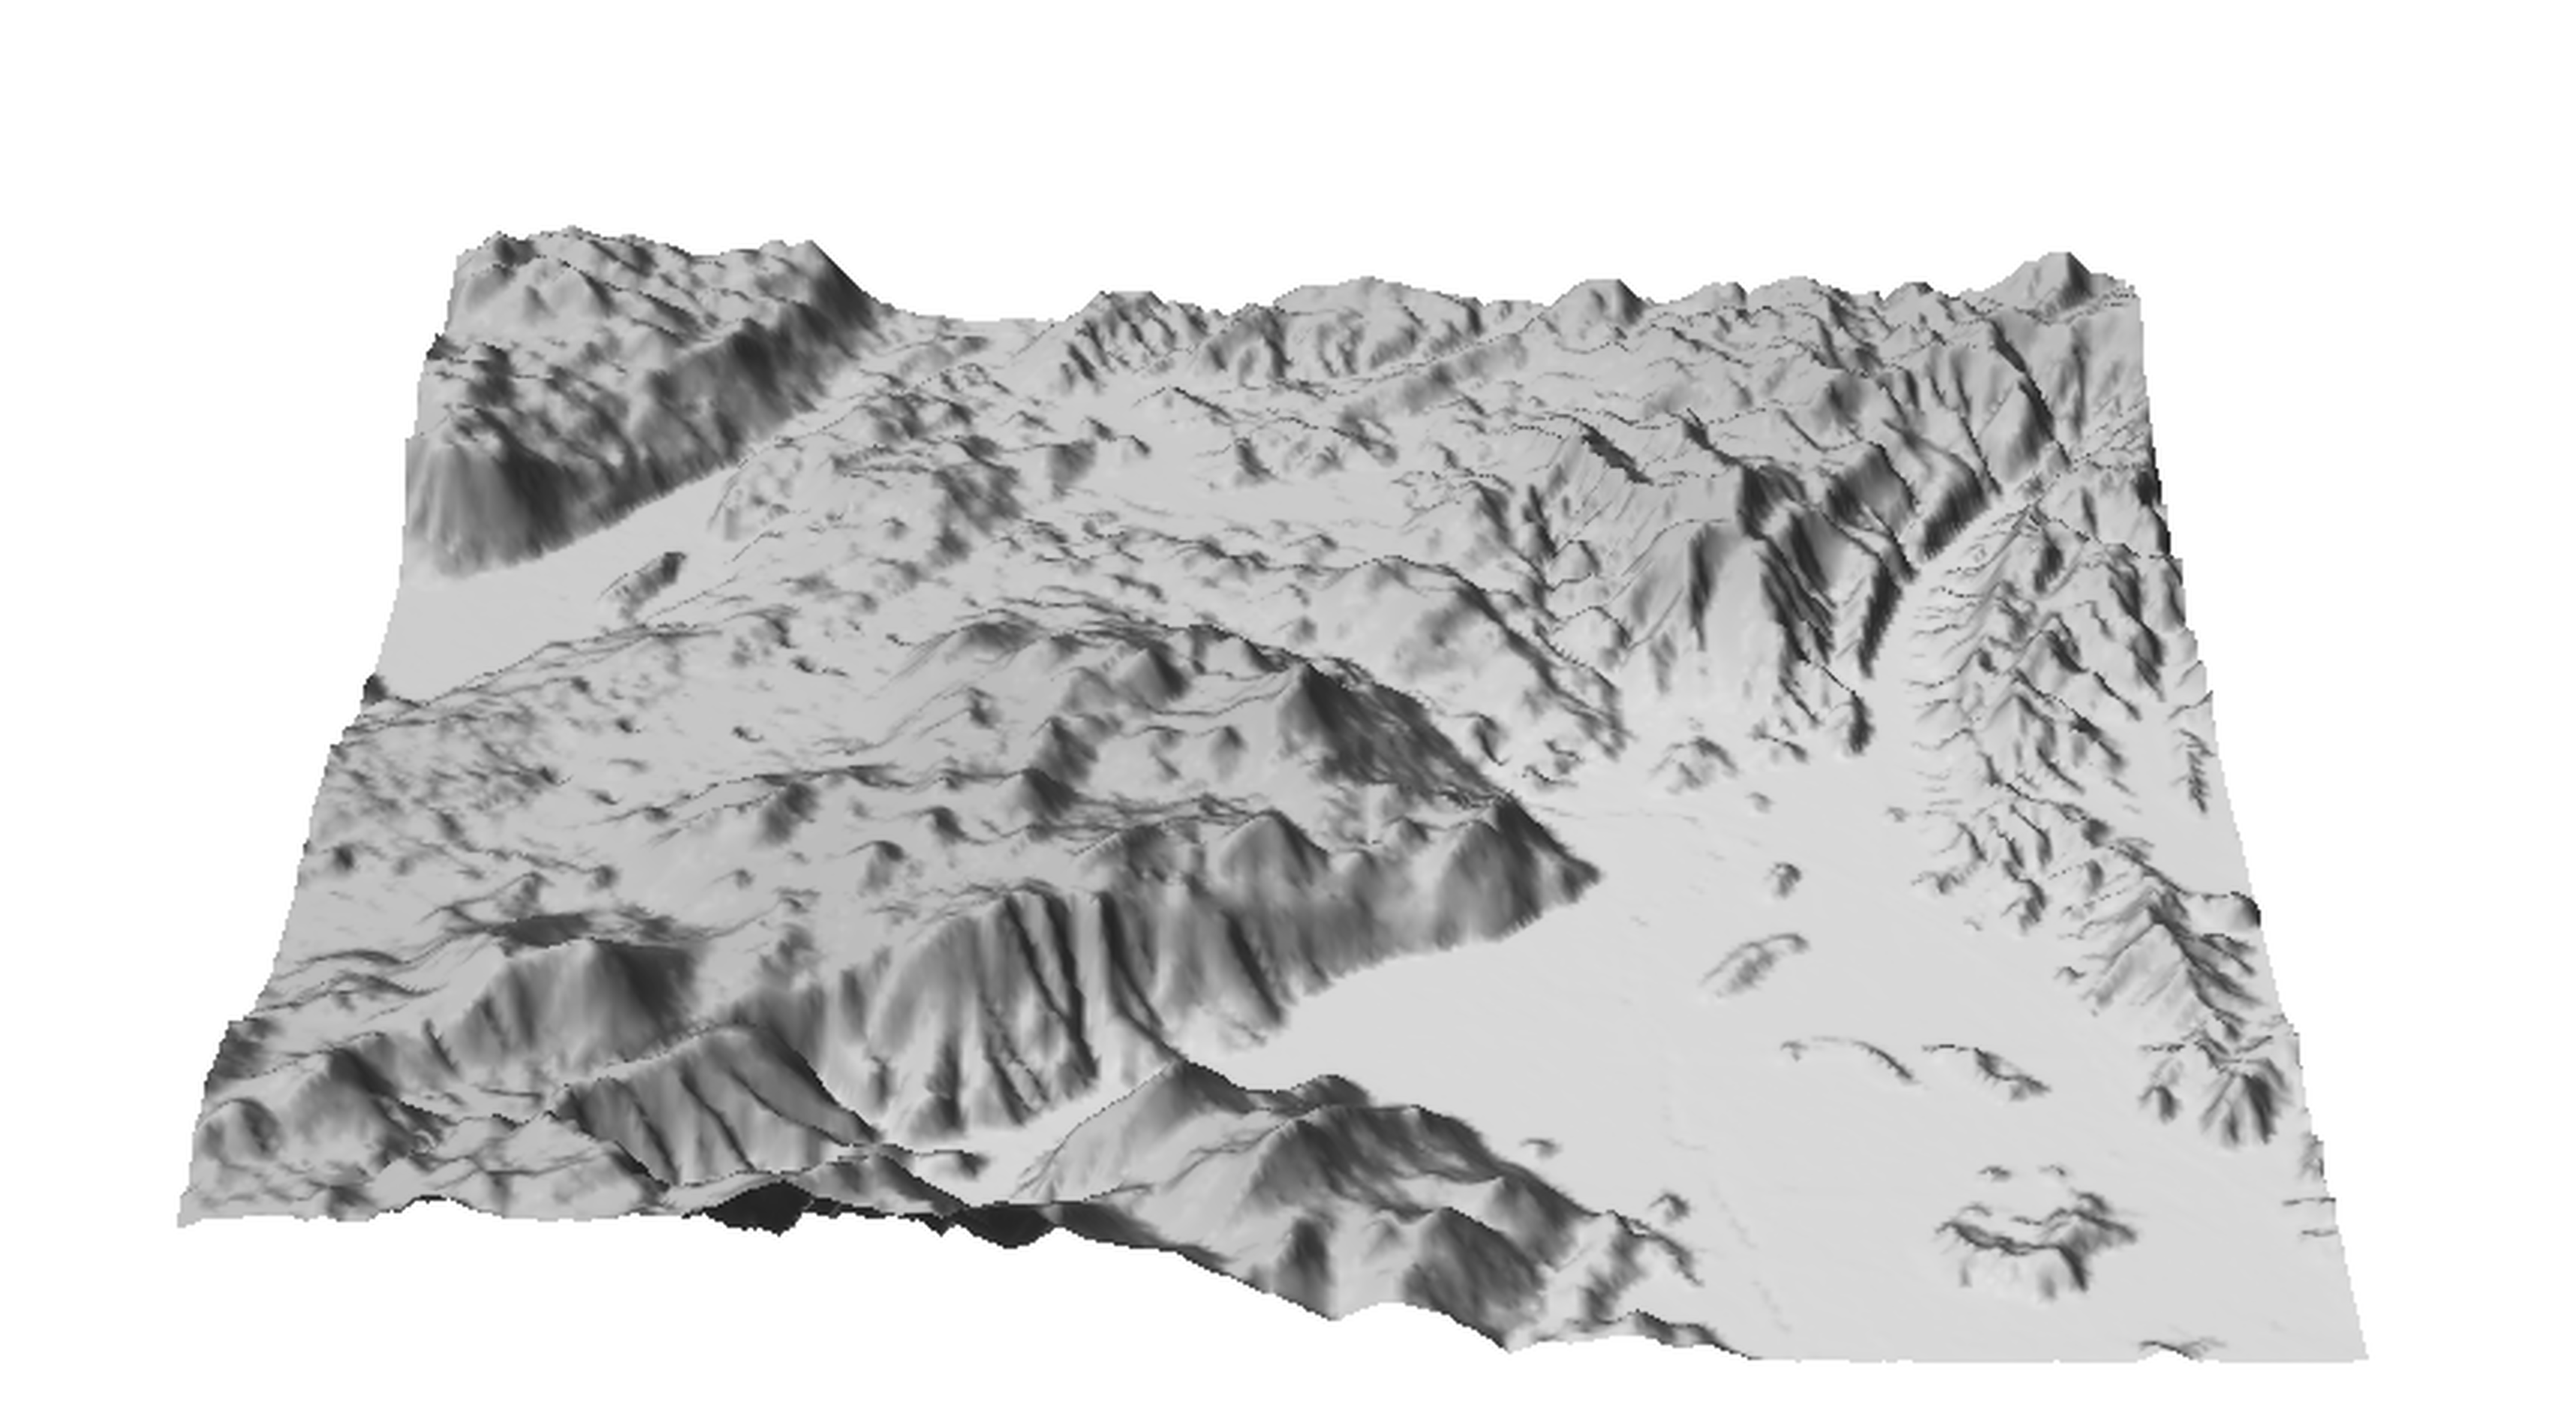
\includegraphics[width=1\columnwidth]{\lyxdot \lyxdot /tun_par/doc/img/terrain_HI}

\caption{Terrain profile for network Net$_{3}$, dominated by hills.\label{fig:terrain_profile-Net3}}
%
\end{minipage}
\end{figure*}



\subsubsection{Test networks \label{sub:Test-networks}}

All the test networks, Net$_{1}$, Net$_{2}$, and Net$_{3}$ are
subsets of a real LTE network deployed in Slovenia by Telekom Slovenije,
d.d. The path-loss predictions are calculated using a digital elevation
model and clutter map of 25~m$^{2}$ resolution and a receiver height
of 1.5~m above ground level. A radius of 16~km is taken around each
network cell, thus limiting the path-loss prediction to a distance
where the it is still feasible for the mobile to connect to a cell,
with a RSRP greater or equal to -124~dBm \cite{Neuland_Influence_of_Different_Factors_on_X_Map_Estimation_in_LTE:2011}.
At the same time, the selected calculation radius provides enough
overlap among neighboring cells to also calculate the network coverage
over the whole region. Table \ref{tab:Test_network_properties} provides
more information about the test networks used.

\begin{table}
\caption{Several properties of the test networks used for the experimental
simulations.\label{tab:Test_network_properties}}


{\footnotesize \centering}{\footnotesize \par}

{\footnotesize }%
\begin{tabular}{ccc>{\centering}p{2.5cm}}
\hline 
 & {\footnotesize Number of cells } & {\footnotesize Area (km$^{2}$)} & {\footnotesize Field-measurement proportion (\%)}\tabularnewline
\hline 
{\footnotesize Net$_{1}$ } & {\footnotesize 12} & {\footnotesize 103.74} & {\footnotesize 5.41}\tabularnewline
{\footnotesize Net$_{2}$ } & {\footnotesize 130 } & {\footnotesize 1298.02} & {\footnotesize 12.02}\tabularnewline
{\footnotesize Net$_{3}$ } & {\footnotesize 6 } & {\footnotesize 386.38} & {\footnotesize 2.30}\tabularnewline
\hline 
\end{tabular}
\end{table}


Net$_{1}$ represents a network deployed over a dominant agricultural
area with almost flat terrain, some forests and waters streams. Net$_{2}$,
on the other hand, is deployed over a densely populated urban area,
containing high buildings, parks and avenues. The last network, Net$_{3}$,
represents a network deployed over hilly terrain, including some smaller
villages and vast forests. It is important to note that the number
of deployed cells is directly related to the population density within
the region of each test network, as the number of cells from Table
\ref{tab:Test_network_properties} show. For a clearer representation
of the test networks used, we present the proportion of each land-usage
(clutter) category in Table \ref{tab:Proportion_of_clutter_for_test_networks}.

The terrain profiles are most relevant for Net$_{1}$ and Net$_{3}$,
since none of them comprehends an urban environment. Note that the
terrain shown in Figure \ref{fig:terrain_profile-Net1} is mostly
flat, since the agricultural area is predominant there. In contrast,
the terrain for Net$_{3}$ is dominated by hills, which are mostly
covered by dense forests, with some small villages in the valleys
(see Figure \ref{fig:terrain_profile-Net3}).


\subsubsection{Experimental environment}

The simulations were carried out on 40 computing nodes of the DEGIMA
cluster \cite{Hamada_Cluster_of_GPUs:2010} at the Nagasaki Advanced
Computing Center (NACC) of the Nagasaki University in Japan. This
system ranked in the TOP 500 list of supercomputers until June 2012%
\footnote{http://www.top500.org%
}, and in June 2011 held the third place of the Green 500 list%
\footnote{http://www.green500.org%
} as one of the most energy-efficient supercomputers in the world.

The computing nodes are connected by a LAN, over a Gigabit Ethernet
interconnect. The reason for using a high-end computer cluster as
DEGIMA is to exploit the parallel nature of PRATO. However, this does
not mean that the presented simulation cannot be carried out serially
in a commodity desktop computer. PRATO does support serial calculation
of radio-propagation predictions for several cells.

Each computing node of DEGIMA features one of two possible configurations,
namely:
\begin{itemize}
\item Intel Core i5-2500T quad-core processor CPU, clocked at 2.30 GHz,
with 16 GB of RAM; and
\item Intel Core i7-2600K quad-core processor CPU, clocked at 3.40 GHz,
also with 16 GB of RAM.
\end{itemize}
During the simulation runs, the nodes equipped with the Intel i5 CPU
host the worker processes, whereas the master process runs on a computing
node featuring an Intel i7 CPU, and performing all its I/O operations
on the local file system.

All the nodes are equipped with a Linux 64-bit operating system (Fedora
distribution). As the message passing implementation we use OpenMPI,
version 1.6.1, which has been manually compiled with the distribution-supplied
gcc compiler, version 4.4.4.


\subsubsection{Results \label{sub:Optimization-results}}

The results of applying the linear least squares method to fit the
parameters of the radio-prediction model to a set of field measurements
presented in this section. We have prepared bar charts showing the
cumulative distribution of the absolute error between the prediction
points and the field measurements. Each bar represents an open interval,
expressed in dB, denoting the proportion of points that deviate from
the prediction for the expressed number of dB. For example, in Figure
\ref{fig:error_distribution_default_parameters-Net1}, we may see
that the proportion of predicted points differing from the field measurements
in 35 dB or more is around 16\%, whereas the proportion differing
in less than 5 dB is 10\%. These numbers represent the test network
Net$_{1}$ before applying the model-parameter fitting. For comparison,
in Figure \ref{fig:error_distribution_optimal_parameters-Net1}, the
absolute-error distribution for the same test network is given, but
with the model parameters fitted to the available field measurements.
Notice how the proportions describing the biggest deviation have dropped
to under 5\% (35 dB and more) and less than 6\% (30 dB to 35 dB).
Moreover, it is clear how all proportions improved, raising the bars
towards the left-hand side.

The error distributions of the radio-propagation prediction for test
network Net$_{2}$ using default parameters and fitted ones are given
in Figures \ref{fig:error_distribution_default_parameters-Net2} and
\ref{fig:error_distribution_optimal_parameters-Net2}, respectively.
In this case, the improvement is even more significant than for the
first test network, clearly showing that the tuned propagation model
represents the local radio propagation conditions within this environment
more accurately.

For the third test network, Net$_{3}$, the error distributions are
depicted in Figure \ref{fig:error_distribution_default_parameters-Net3}
using the default parameters, and Figure \ref{fig:error_distribution_optimal_parameters-Net3}
for the tinned ones. Similarly as for the first test network, Net$_{1}$,
we may see a how the proportion of highest error deviation has been
lowered over those with lower deviation values. 

The overall results confirm that fitting the parameters of the radio-propagation
model to the field measurements within a certain region significantly
improve the quality of the calculated propagation prediction.

Despite the presented results are encouraging, there are some specific
reasons behind the considerable better results for Net$_{2}$, when
compared to those of Net$_{1}$ and Net$_{2}$. Clearly, the number
of available field measurements directly affects the quality of the
calculated results, making the least squares approximation rougher
and thus less precise (see Table \ref{tab:Test_network_properties}
in Section \ref{sub:Test-networks}). However, it is out of the scope
of this work, in which we focus is on the applicability of PRATO as
a tool for planning and optimization of LTE networks, to assess the
quality of the achieved results. Nevertheless, for the sake of completeness,
we would like to point out that some researchers have already started
working on different ways on how to improve this aspect \cite{Neuland_Influence_of_Different_Factors_on_X_Map_Estimation_in_LTE:2011,Neuland_Influence_of_positioning_error_on_X_Map_estimation_in_LTE:2011}.

\begin{figure*}
\begin{minipage}[t]{0.49\textwidth}%
\centering

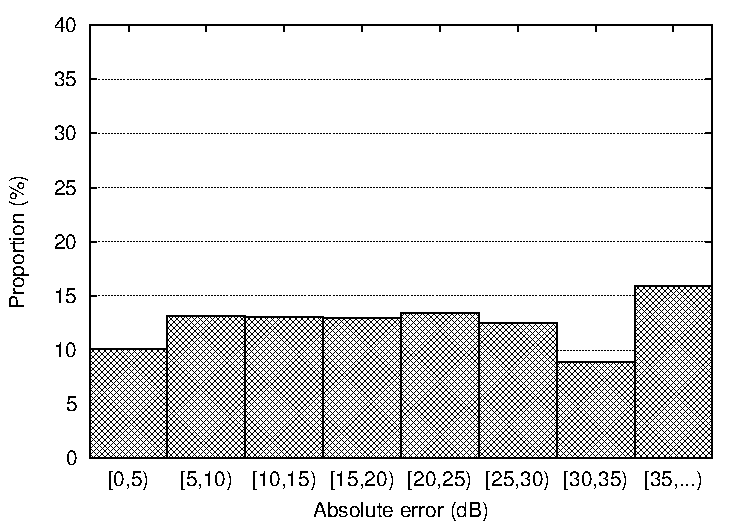
\includegraphics[width=0.8\columnwidth]{\lyxdot \lyxdot /tun_par/doc/img/error_distribution-MS-def_params}

\caption{Error distribution of the radio prediction for network Net$_{1}$
with default parameter values.\label{fig:error_distribution_default_parameters-Net1}}
%
\end{minipage}\hfill{}%
\begin{minipage}[t]{0.49\textwidth}%
\centering

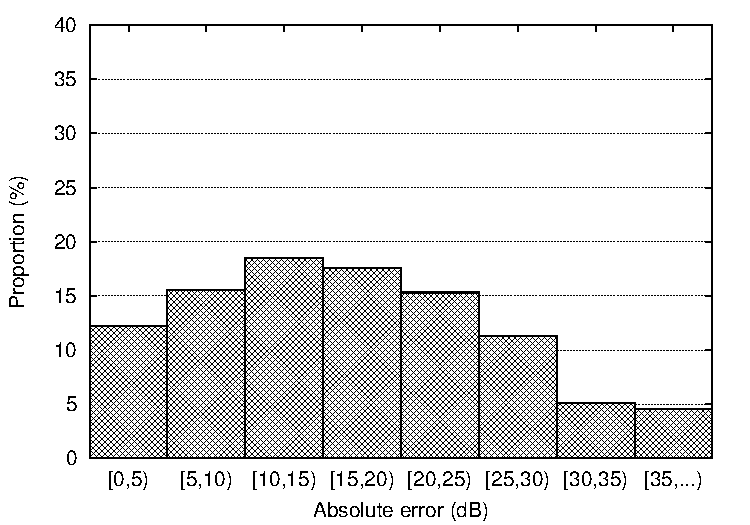
\includegraphics[width=0.8\columnwidth]{\lyxdot \lyxdot /tun_par/doc/img/error_distribution-MS-opt_params}

\caption{Error distribution of the radio prediction for network Net$_{1}$
with fitted parameter values.\label{fig:error_distribution_optimal_parameters-Net1}}
%
\end{minipage}
\end{figure*}


\begin{figure*}
\begin{minipage}[t]{0.49\textwidth}%
\centering

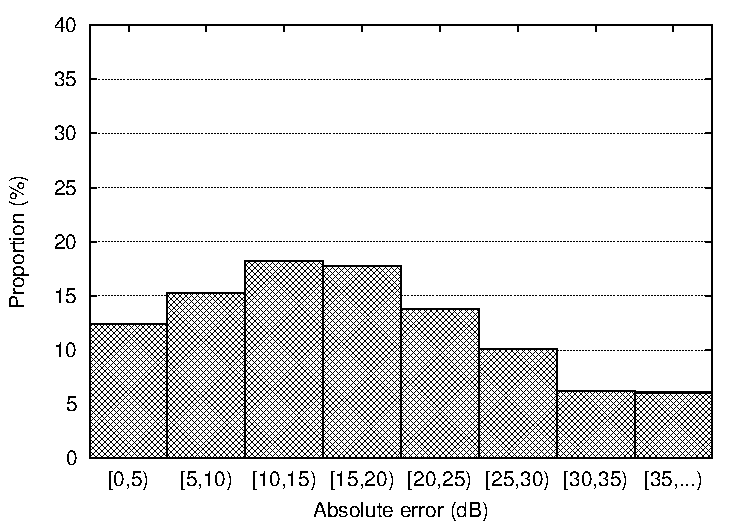
\includegraphics[width=0.8\columnwidth]{\lyxdot \lyxdot /tun_par/doc/img/error_distribution-LJ-opt_params}

\caption{Error distribution of the radio prediction for network Net$_{2}$
with default parameter values.\label{fig:error_distribution_default_parameters-Net2}}
%
\end{minipage}\hfill{}%
\begin{minipage}[t]{0.49\textwidth}%
\centering

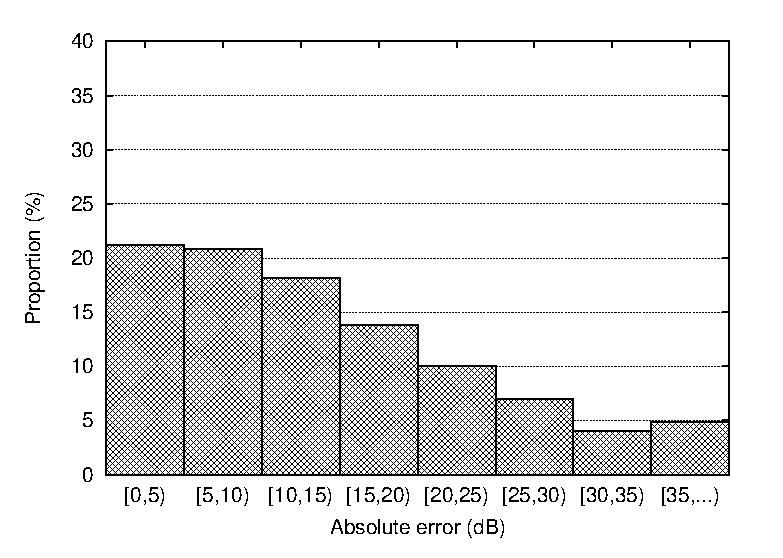
\includegraphics[width=0.8\columnwidth]{\lyxdot \lyxdot /tun_par/doc/img/error_distribution-LJ-def_params}

\caption{Error distribution of the radio prediction for network Net$_{2}$
with fitted parameter values.\label{fig:error_distribution_optimal_parameters-Net2}}
%
\end{minipage}
\end{figure*}


\begin{figure*}
\begin{minipage}[t]{0.49\textwidth}%
\centering

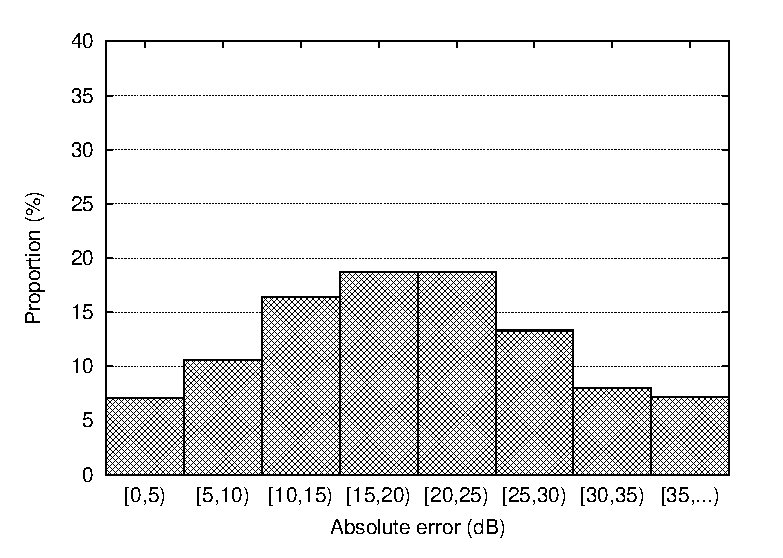
\includegraphics[width=0.8\columnwidth]{\lyxdot \lyxdot /tun_par/doc/img/error_distribution-HI-def_params}

\caption{Error distribution of the radio prediction for network Net$_{3}$
with default parameter values.\label{fig:error_distribution_default_parameters-Net3}}
%
\end{minipage}\hfill{}%
\begin{minipage}[t]{0.49\textwidth}%
\centering

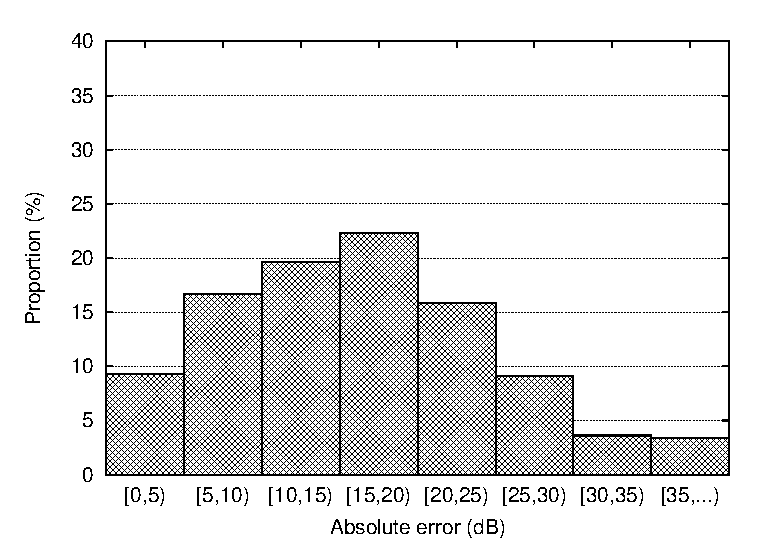
\includegraphics[width=0.8\columnwidth]{\lyxdot \lyxdot /tun_par/doc/img/error_distribution-HI-opt_params}

\caption{Error distribution of the radio prediction for network Net$_{3}$
with fitted parameter values.\label{fig:error_distribution_optimal_parameters-Net3}}
%
\end{minipage}
\end{figure*}



\section{Clutter optimization}\label{sec:Clutter-optimization}

In order to better adapt the radio-prediction calculation to a given
regional environment, the signal losses due to clutter have to be
optimized. As it was mentioned before, there are several reasons for
the signal loss values to be inaccurate. Among them, we can mention
seasonal changes, like tree foliage or snow, construction or demolition
of buildings and parks, different kinds of forests or agricultural
areas. These changes are only noticeable through regular field-measurement
campaigns and land-usage data updates. The challenge is thus to combine
both in order to improve the prediction results even further.

In the following, we use a metaheuristic algorithm in order to optimize
the clutter losses, i.e. the signal loss due to terrain influence,
of several regions within the mobile network under optimization. This
is done over a group of network cells within different regions of
the target network, e.g. agricultural, urban or hilly. In terms of
radio-network planning, a regional classification of signal loss due
to clutter further improve the accuracy of the radio-coverage prediction,
thus enhancing the model by distinguishing, for example, different
types of agricultural, park and vegetation areas.

Compared to the parameter tuning of the mathematical model presented
in Section \ref{sub:Radio-prediction-model}, we are not using an
analytical approach for tackling this problem, since we wish to potentially
include corrections for possible errors in the NLOS part Equation
\ref{eq:eric_pathloss}. For this reason, we turn our attention to
metaheuristic algorithms \cite{Talbi_Metaheuristics:2009} in general
and swarm intelligence in particular \cite{Kennedy_Swarm_intelligence:2006}.
From this last family of metaheuristic algorithms, we choose the differential
ant-stigmergy algorithm (DASA) \cite{Korosec-The_differential_ant_stigmergy_algorithm:2012}.

Several authors have shown the benefits of using metaheuristic algorithms
for tackling radio-related problems \cite{Benedicic_Balancing_downlink_uplink_soft_handover_areas_in_UMTS_networks:2012,Garcia-Lozano_Metaheuristic_procedure_to_optimize_transmission_delays_in_DVB-T_single_frequency_networks:2011,Huang_Online_propagation_model_correction_based_on_PSO_algorithm_in_LTE_SON_system:2012,Malla_Energy_efficient_resource_allocation_in_OFDMA_networks_using_ant_colony_optimization:2012}.
In our case, an analytical approach may also be possible, but our
objective is to show the capabilities of PRATO when combining an optimization
algorithm with parallel and distributed objective-function evaluation.
For the following simulations, the DASA runs as the master process,
whereas the workers evaluate the current solution in parallel for
all the involved cells (see Figure \ref{fig:PRATO_architecture_optimization}).


\subsection{Optimization objective \label{sub:Optimization-objective}}

The optimization objective consists of adjusting the loss values of
the different clutter categories, i.e. $pl_{\mathrm{CLUT}}(d_{(x,y)})$
of Equation (\ref{eq:eric_pathloss}), to best fit a set of field
measurements in a given region containing multiple cells. We have
three data sets at our disposal, one for each of the three regions:
the first for Net$_{1}$, the second for Net$_{2}$, and the third
for Net$_{3}$. Each region is independently optimized, so that the
radio-propagation predictions of its network cells, which already
have their model parameters fitted, minimize the mean-squared error
against the field measurements, namely

\begin{multline}
F^{*}(R)=\sum_{i=1}^{m_{c}}\frac{(p_{c}-pl_{c}(d_{(x,y)},\beta_{c})-fm_{i})^{2}}{m_{R}}\;\forall c\in R,\label{eq:mean_squared_error}
\end{multline}


\noindent where $F^{*}(R)$ is the optimization objective to be minimized,
$R$ is one of the three regions, $p_{c}$ is the transmit power of
cell $c$, $fm_{i}$ is the $i$-th field measurement out of a set
of measurements of cell $c$ with cardinality $m_{c}$, $m_{R}$ is
the number of field measurements of all the cells within the region
$R$, and $pl_{c}(d_{(x,y)},\beta)$ is the path loss of cell $c$
at coordinate $(x,y)$, where $\beta$ contains per-cell fitted parameter
values of the prediction model.

For a reference of the different clutter categories our prediction
model recognizes, see Table \ref{tab:Clutter-categories}.


\subsection{Differential ant-stigmergy algorithm}

As it has been mentioned before, the optimization algorithm we have
chosen for the clutter-optimization problem is the (DASA). Based on
the metaheuristic Ant-Colony Optimization (ACO) \cite{Dorigo_Ant_colony_optimization:2006},
the DASA \cite{Korosec-The_differential_ant_stigmergy_algorithm:2012}
provides a framework to successfully cope with high-dimensional numerical
optimization problems. It creates a fine-grained discrete form of
the search space, representing it as a graph. This graph is then used
as the walking paths for the ants, which iteratively improve the temporary
best solution.

The mapping between the clutter-optimization problem and DASA is as
follows:

\begin{equation}
X_{a}=\left\{ x_{1},x_{2},\ldots x_{i},\ldots,x_{12}\right\} \label{eq:DASA-problem_mapping}
\end{equation}


\noindent where $X_{a}$ is the solution vector of ant $a$ during
the minimization process, and $x_{i}$ represents the $i$-th clutter
category within a given region. At the end of every iteration, and
after all the ants have created solutions, they are evaluated to establish
if any of them is better than the best solution found so far.

There are six parameters that control the way DASA explores the search
space: the number of ants, the discrete base, the pheromone dispersion
factor, the global scale-increasing factor, the global scale-decreasing
factor, and the maximum parameter precision.

For a more in-depth explanation about these parameters and the DASA
algorithm itself, we refer the reader to \cite{Korosec-The_differential_ant_stigmergy_algorithm:2012}.


\subsection{Simulations}

In this case, the simulations for each test network comprise multiple
iterations of several steps. An iteration begins by generating a solution
vector for each of the ants in the DASA population. The following
step involves the parallel evaluation of each solution, i.e. one radio-coverage
prediction per cell. The final step is calculating the objective-function
value, as defined in Equation (\ref{eq:mean_squared_error}), before
sending it to the DASA for it to generate the next set of solutions.
Figure \ref{fig:PRATO_architecture_optimization} depicts the way
PRATO performs the objective-function evaluation in parallel over
the worker processes, while the optimization algorithm runs on the
master one.

\begin{figure}
\centering

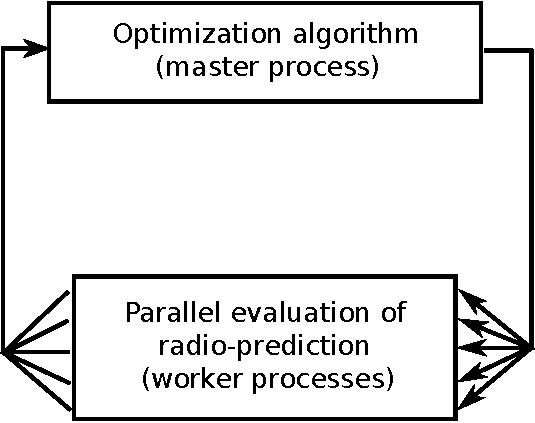
\includegraphics[width=0.6\columnwidth]{\lyxdot \lyxdot /tun_par/doc/img/architecture}

\caption{\textit{PRATO architecture and data flow during the clutter-optimization
phase.\label{fig:PRATO_architecture_optimization}}}
\end{figure}


Compared to the experiments presented in Section \ref{sub:Simulations},
a much higher number of evaluations is needed for this kind of optimization.
In this context, it is of key importance to perform the radio-coverage
prediction for multiple cells in a parallel manner. Otherwise, such
an approach would not be feasible, since the time required to reach
a reasonable solution would be excessive.

The loss value (in dB) each clutter category may take has been limited
to the interval {[}0,40{]}. This information has been provided by
the radio experts of the Radio Network department at Telekom Slovenije,
d.d.

As stopping criteria of the optimization runs for Net$_{1}$ and Net$_{3}$,
we have fixed the maximum number of iterations to 200, whereas for
Net$_{2}$ this values has been set to 500 iterations, since this
networks comprises the largest number of network cells. Overall, the
framework completed 48,000 objective-function evaluations in the former
case, and 120,000 in the latter one.

Regarding the parameters that control algorithm behavior, we have
set them to the following values
\begin{itemize}
\item $m=240$, the number of ants;
\item $b=10,$ the discrete base;
\item $q=0.2$, the pheromone dispersion factor;
\item $s_{+}=0.01$, the global scale-increasing factor;
\item $s_{-}=0.01$, the global scale-decreasing factor; and 
\item $e=1.0^{-2}$, the maximum parameter precision.
\end{itemize}

\subsection{Results}

\begin{table}
\caption{Clutter-category losses after the optimization. The default losses
for each clutter category are given along the solutions for each of
the test networks. All values are expressed in dB. \label{tab:Clutter-optimization-solutions}}


{\footnotesize \centering}{\footnotesize \par}

{\footnotesize }%
\begin{tabular}{ccccc}
\hline 
{\footnotesize Clutter category} & {\footnotesize Default} & {\footnotesize Net$_{1}$} & {\footnotesize Net$_{2}$} & {\footnotesize Net$_{3}$}\tabularnewline
\hline 
{\footnotesize 0} & {\footnotesize 5.0} & {\footnotesize 13.71} & {\footnotesize 11.30} & {\footnotesize 17.90}\tabularnewline
{\footnotesize 1} & {\footnotesize 15.0} & {\footnotesize 12.39} & {\footnotesize 16.67} & {\footnotesize -}\tabularnewline
{\footnotesize 2} & {\footnotesize 13.0} & {\footnotesize 16.04} & {\footnotesize 17.04} & {\footnotesize 15.69}\tabularnewline
{\footnotesize 3} & {\footnotesize 28.0} & {\footnotesize 19.59} & {\footnotesize 18.01} & {\footnotesize 23.00}\tabularnewline
{\footnotesize 4} & {\footnotesize 12.0} & {\footnotesize 11.48} & {\footnotesize 9.71} & {\footnotesize 10.80}\tabularnewline
{\footnotesize 5} & {\footnotesize 20.0} & {\footnotesize 16.26} & {\footnotesize 11.62} & {\footnotesize 16.26}\tabularnewline
{\footnotesize 6} & {\footnotesize 15.0} & {\footnotesize -} & {\footnotesize -} & {\footnotesize -}\tabularnewline
{\footnotesize 7} & {\footnotesize 8.0} & {\footnotesize -} & {\footnotesize 13.49} & {\footnotesize -}\tabularnewline
{\footnotesize 8} & {\footnotesize 5.0} & {\footnotesize -} & {\footnotesize 13.50} & {\footnotesize -}\tabularnewline
{\footnotesize 9} & {\footnotesize 1.0} & {\footnotesize 17.50} & {\footnotesize 5.60} & {\footnotesize -}\tabularnewline
{\footnotesize 10} & {\footnotesize 20.0} & {\footnotesize 8.26} & {\footnotesize 16.75} & {\footnotesize 16.63}\tabularnewline
{\footnotesize 11 } & {\footnotesize 8.0} & {\footnotesize -} & {\footnotesize 18.93} & {\footnotesize -}\tabularnewline
\hline 
\end{tabular}
\end{table}


The results calculated by the optimization process are shown in Table
\ref{tab:Clutter-optimization-solutions}. The solutions are given
for each of the test networks, along with typical default loss values
due to clutter. Hyphens represent clutter categories for which there
are no field measurements available. Consequently, it is not possible
to calculate an objective-function value for them.

The optimized loss for the first clutter category, 0, representing
urban area without buildings, is larger than the default value in
all three networks. This may be attributed to the fact that ...???
As for the category 1, representing suburban area, the value for Net$_{1}$
is lower than the default one, mainly because this network is deployed
over a predominant agricultural area, i.e. suburban areas are less
dense here. On the other hand, the value for Net$_{2}$ is larger,
indicating a building density above the average, whereas for Net$_{3}$,
the value could not be calculated due to lack of measurements. A similar
behavior may be observed for category 2, representing urban area.
However, for category 3, representing dense urban area, the optimized
losses of all three networks are lower than the default value, indicating
dense urban areas here are not as dense as the average case. Representing
agricultural area, category 4 gets a value very close to the default
one for Net$_{1}$ and Net$_{3}$, whereas for Net$_{2}$ the value
is lower, indicating the most of this kind of land is not being exploited
near the city. As for category 5, representing forests, the results
are well corresponded with the kind of forest dominating each of the
test networks, being those of Net$_{1}$ and Net$_{3}$ more dense
due to leave foliage, whereas as for Net$_{2}$ the forests are mostly
coniferous and more sparse. Keeping the default loss values for categories
6, 7 and 8, we move on to category 9, representing water, for which
the results of all three networks indicate creeks and rivers in these
areas are mostly surrounded by forests (Net$_{1}$) or buildings (Net$_{2}$),
since none of the regions lays by the sea. As for the industrial areas,
denoted by clutter category 10, show lower loss values than the typical
default, indicating very sparse industrial buildings (Net$_{1}$)
and a higher density of mostly commercial buildings for Net$_{2}$
and Net$_{3}$).

These results clearly show the benefit of the optimization of losses
due to land usage or clutter, by finely adapting these values to local
conditions within the environment where these networks are deployed.


\subsubsection{Statistical analysis}

Because of the stochastic nature of the optimization algorithm, we
have collected the results from 30 independent runs, in order to have
enough data for the results to be statistically relevant. In other
words, the robustness of the solutions presented in the previous section
is analyzed here.

To this end, Table \ref{tab:Solutions-analysis} shows the solutions
reached by the DASA for each of three test networks. The calculated
signal losses are thus depicted with the minimum, maximum and average
values for every clutter category, along with their standard deviation.
Similarly as before, hyphens represent clutter categories for which
there are no field measurements available, and thus they cannot be
optimized. 

\begin{table*}
\caption{Statistical analysis of the optimization solutions for each test network.
All values are expressed in dB. \label{tab:Solutions-analysis}}


{\footnotesize \centering}{\footnotesize \par}

\begin{tabular}{cccccccccccccccc}
\cline{3-16} 
 &  &  & Net$_{1}$ &  &  &  &  & Net$_{2}$ &  &  &  &  & Net$_{3}$ &  & \tabularnewline
\hline 
{\footnotesize Category} &  & {\footnotesize Min} & {\footnotesize Max} & {\footnotesize Avg} & {\footnotesize St.dev.} &  & {\footnotesize Min} & {\footnotesize Max} & {\footnotesize Avg} & {\footnotesize St.dev.} &  & {\footnotesize Min} & {\footnotesize Max} & {\footnotesize Avg} & {\footnotesize St.dev.}\tabularnewline
\hline 
{\footnotesize 0} &  & {\footnotesize 13.36} & {\footnotesize 13.97} & {\footnotesize 13.71} & {\footnotesize 0.15} &  & {\footnotesize 11.22} & {\footnotesize 11.40} & {\footnotesize 11.30} & {\footnotesize 0.04} &  & {\footnotesize 17.72} & {\footnotesize 17.85} & {\footnotesize 17.90} & {\footnotesize 0.07}\tabularnewline
\cline{1-6} \cline{8-11} \cline{13-16} 
{\footnotesize 1} &  & {\footnotesize -} & {\footnotesize -} & {\footnotesize -} & {\footnotesize -} &  & {\footnotesize 14.25} & {\footnotesize 19.20} & {\footnotesize 16.67} & {\footnotesize 1.87} &  & {\footnotesize -} & {\footnotesize -} & {\footnotesize -} & {\footnotesize -}\tabularnewline
\cline{1-6} \cline{8-11} \cline{13-16} 
{\footnotesize 2} &  & {\footnotesize 15.84} & {\footnotesize 16.21} & {\footnotesize 16.04} & {\footnotesize 0.08} &  & {\footnotesize 16.99} & {\footnotesize 17.11} & {\footnotesize 17.04} & {\footnotesize 0.03} &  & {\footnotesize 15.64} & {\footnotesize 15.72} & {\footnotesize 15.69} & {\footnotesize 0.03}\tabularnewline
\cline{1-6} \cline{8-11} \cline{13-16} 
{\footnotesize 3} &  & {\footnotesize 19.15} & {\footnotesize 20.07} & {\footnotesize 19.59} & {\footnotesize 0.25} &  & {\footnotesize 17.95} & {\footnotesize 18.12} & {\footnotesize 18.01} & {\footnotesize 0.04} &  & {\footnotesize 22.68} & {\footnotesize 23.20} & {\footnotesize 23.00} & {\footnotesize 0.16}\tabularnewline
\cline{1-6} \cline{8-11} \cline{13-16} 
{\footnotesize 4} &  & {\footnotesize 11.35} & {\footnotesize 11.62} & {\footnotesize 11.48} & {\footnotesize 0.05} &  & {\footnotesize 9.63} & {\footnotesize 9.77} & {\footnotesize 9.71} & {\footnotesize 0.03} &  & {\footnotesize 10.73} & {\footnotesize 10.84} & {\footnotesize 10.80} & {\footnotesize 0.03}\tabularnewline
\cline{1-6} \cline{8-11} \cline{13-16} 
{\footnotesize 5} &  & {\footnotesize 16.00} & {\footnotesize 16.54} & {\footnotesize 16.26} & {\footnotesize 0.14} &  & {\footnotesize 11.45} & {\footnotesize 11.80} & {\footnotesize 11.62} & {\footnotesize 0.08} &  & {\footnotesize 16.19} & {\footnotesize 16.30} & {\footnotesize 16.26} & {\footnotesize 0.04}\tabularnewline
\cline{1-6} \cline{8-11} \cline{13-16} 
{\footnotesize 6} &  & {\footnotesize -} & {\footnotesize -} & {\footnotesize -} & {\footnotesize -} &  & {\footnotesize -} & {\footnotesize -} & {\footnotesize -} & {\footnotesize -} &  & {\footnotesize -} & {\footnotesize -} & {\footnotesize -} & {\footnotesize -}\tabularnewline
\cline{1-6} \cline{8-11} \cline{13-16} 
{\footnotesize 7} &  & {\footnotesize -} & {\footnotesize -} & {\footnotesize -} & {\footnotesize -} &  & {\footnotesize 12.71} & {\footnotesize 14.52} & {\footnotesize 13.49} & {\footnotesize 0.39} &  & {\footnotesize -} & {\footnotesize -} & {\footnotesize -} & {\footnotesize -}\tabularnewline
\cline{1-6} \cline{8-11} \cline{13-16} 
{\footnotesize 8} &  & {\footnotesize -} & {\footnotesize -} & {\footnotesize -} & {\footnotesize -} &  & {\footnotesize 12.25} & {\footnotesize 15.79} & {\footnotesize 13.50} & {\footnotesize 0.83} &  & {\footnotesize -} & {\footnotesize -} & {\footnotesize -} & {\footnotesize -}\tabularnewline
\cline{1-6} \cline{8-11} \cline{13-16} 
{\footnotesize 9} &  & {\footnotesize 16.07} & {\footnotesize 18.80} & {\footnotesize 17.50} & {\footnotesize 0.83} &  & {\footnotesize 4.67} & {\footnotesize 6.26} & {\footnotesize 5.60} & {\footnotesize 0.35} &  & {\footnotesize -} & {\footnotesize -} & {\footnotesize -} & {\footnotesize -}\tabularnewline
\cline{1-6} \cline{8-11} \cline{13-16} 
{\footnotesize 10} &  & {\footnotesize 7.79} & {\footnotesize 8.54} & {\footnotesize 8.26} & {\footnotesize 0.19} &  & {\footnotesize 16.68} & {\footnotesize 16.87} & {\footnotesize 16.75} & {\footnotesize 0.05} &  & {\footnotesize 16.50} & {\footnotesize 16.68} & {\footnotesize 16.63} & {\footnotesize 0.07}\tabularnewline
\cline{1-6} \cline{8-11} \cline{13-16} 
{\footnotesize 11} &  & {\footnotesize -} & {\footnotesize -} & {\footnotesize -} & {\footnotesize -} &  & {\footnotesize 18.62} & {\footnotesize 19.20} & {\footnotesize 17.04} & {\footnotesize 0.13} &  & {\footnotesize -} & {\footnotesize -} & {\footnotesize -} & {\footnotesize -}\tabularnewline
\hline 
\end{tabular}
\end{table*}


\begin{figure*}[tp]
\centering

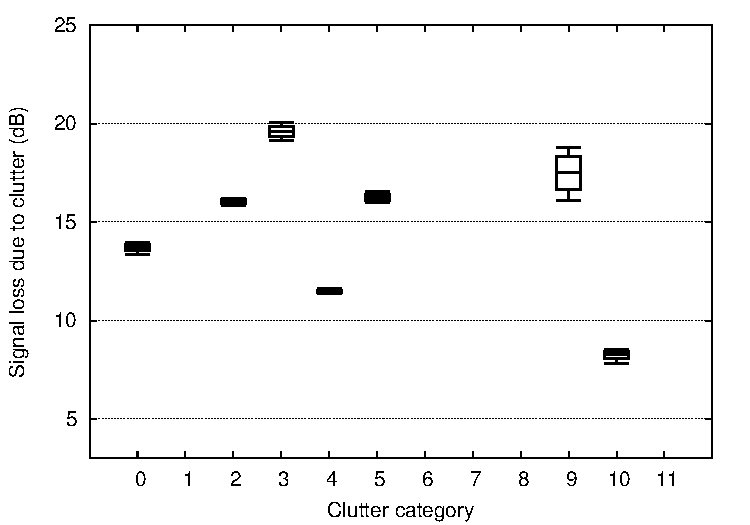
\includegraphics[width=0.49\textwidth]{\lyxdot \lyxdot /tun_par/doc/img/boxplot-MS}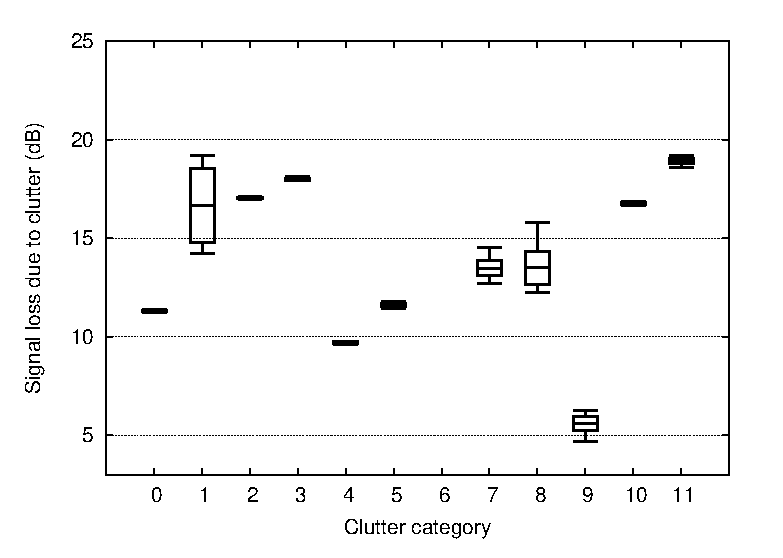
\includegraphics[width=0.49\textwidth]{\lyxdot \lyxdot /tun_par/doc/img/boxplot-LJ}\\\hspace*{0.2in}(a)\hspace*{3.2in}(b)
\end{figure*}


\begin{figure*}[tp]
\centering

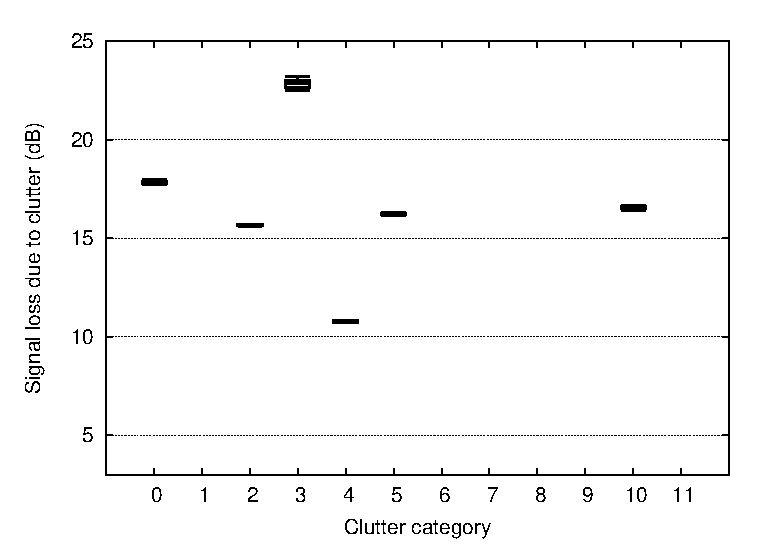
\includegraphics[width=0.51\textwidth]{\lyxdot \lyxdot /tun_par/doc/img/boxplot-HI}\\\hspace*{0.2in}(c)

\caption{Box plots showing the statistical analysis values of Table \ref{tab:Solutions-analysis},
showing the solutions of the clutter-optimization process for each
test network: (a) Net$_{1}$; (b) Net$_{2}$; (c) Net$_{3}$.\label{fig:boxplot}}
\end{figure*}



\section{Related work}\label{sec:Related-work}

There are a few examples of radio-network simulators available for
LTE \cite{Mehlfuhrer_The_Vienna_LTE_Simulators_enabling_reproducibility_in_wireless_communications_research:2011,Piro_Simulating_LTE_cellular_systems_an_open_source_framework:2011,Sanchez_Performance_evaluation_of_OFDMA_wireless_systems_using_WM_SIM:2006},
mostly developed for academic environments, they are not targeted
at real-world environments. A Matlab-based LTE simulator has been
proposed in \cite{Mehlfuhrer_The_Vienna_LTE_Simulators_enabling_reproducibility_in_wireless_communications_research:2011}.
It implements a standard LTE downlink physical layer, including Adaptive
Modulation and Coding (AMC), multiple users, MIMO transmission and
scheduler. Despite being open source and freely available, the fact
of being implemented in Matlab make it very restrictive in terms of
tackling bigger problem instances of real networks. A promising tool
in this sense is presented in \cite{Piro_Simulating_LTE_cellular_systems_an_open_source_framework:2011},
where the authors implement a full-stack LTE system in C++. Although
the tool has no capability for graphically displaying the simulations,
it could be implemented, since the source code is available. In our
opinion, the main drawback of this tool is the lack of documentation,
which makes it very time-consuming to continue extending this work
without the direct help of one of the original authors. In \cite{Ozimek_Open.source.radio.coverage.prediction:2010},
the authors present a tool for radio-coverage calculations of wireless
networks. Implemented as a module of the open-source GRASS system,
it made an ideal basis for expanding it with parallel-computation
capabilities.

As an extension to the well-known NS-2 network simulator, Filiposka
and Trajanov \cite{Filiposka_Terrain_aware_three_dimensional_radio_propagation_model_extension_for_NS2:2011}
introduced a module for radio-propagation predictions, which takes
the terrain profile into account. In this case, the authors focus
on the relief and leave out signal loss due to land-usage, which is
a key factor for acquiring more realistic radio-propagation predictions.

Following an optimization-oriented approach \cite{Aarnaes-Tuning_of_empirical_radio_propagation_models_effect_of_location_accuracy:2004},
the authors study the effects of the location accuracy while performing
a semi-automatic optimization of the parameters of a radio-propagation
model. When compared to our work, where we take a fully automatic
optimization approach, the advantage is clear, since no human intervention
is needed during the optimization process. Besides, they conclude
that locations with a median accuracy of around 60~mts, may be used
for parameter tuning. In this sense, the GPS-informed location of
the field measurements we had available, has been tested to be within
this limit.


\section{Sumary}

We have presented an open-source simulation framework for planning
and optimization of radio networks (PRATO). Based on extensive experimental
simulations, we have shown the suitability of PRATO by tackling two
planning and optimization cases, tested over the newly deployed LTE
network in Slovenia. The first one involved the parameter tuning of
an empirical radio-propagation model using a snapshot of field measurements.
The other one consisted in optimizing the clutter losses over different
regions of the country, therefore adapting the losses due to land
usage to the local conditions of each region.

The encouraging results indicate that PRATO is applicable in planning
and optimization of real-world radio networks in general, and LTE
in particular. Moreover, even computational intensive tasks such as
stochastic optimization, involving thousands of radio-prediction evaluations,
are feasible thanks to the parallelization capabilities provided by
the framework.


\section*{Acknowledgments}

The authors would like to especially thank the staff at the Nagasaki
Advanced Computing Center (NACC) of the Nagasaki University for their
support while making the computer cluster DEGIMA available for the
experimental simulations used in this work. We are also grateful with
the radio engineers at Telekom Slovenije, d.d., for supplying the
network data sets and sharing their professional expertise throughout
the creation of this work.

This project was co-financed by the European Union, through the European
Social Fund.
